69. $y=\cfrac{2x^2-8x}{|x-2|-2}=\begin{cases}\cfrac{2x(x-4)}{x-4}=2x,\ x\geqslant2,\ x\neq4,\\ \cfrac{2x(x-4)}{-x}=8-2x,\ x<2,\ x\neq0.\end{cases}$
$$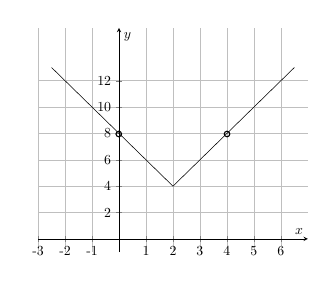
\begin{tikzpicture}[scale=0.5]
\begin{axis}[
    axis lines = middle,
    grid=major,
    legend pos={south west},
    xlabel = {$x$},
    %xlabel style={below right},
    ylabel = {$y$},
    ymin=-1,
    ymax=16,
    xmin=-3,
    xmax=7,
    xtick={-3,-2,-1,1,2,3,4,5,6},
    xticklabels={-3,-2,-1,1,2,3,4,5,6},
    ytick={2,4,6,8,10,12},
    yticklabels={2,4,6,8,10,12},
                  ]
	\addplot[domain=-2.5:2, samples=100, color=black] {2*(4-x)};
    \addplot[domain=2:6.5, samples=100, color=black] {(2*x)};
        %\addplot[domain=2.01:6, samples=100, color=black] {2/(2-x)};
   % \addplot[domain=-3:3, samples=100, color=black] {-x};
     %\addlegendentry{$\text{Рис. 1}$};
\end{axis}
\draw (2.05,3) circle (2pt);
\draw (4.8,3) circle (2pt);
\end{tikzpicture}$$
По графику найдём значение $y=4.$\\
